\section{ViSIT Metadaten und die Semantische Datenbank}\label{sec:semantics}

Brainstorm, things to write about:

\begin{itemize}
	\item theoretischer background: rdf daten, CIDOC, Vismo
	\item datenbank: infrastruktur (hosting, allgemeiner zugriff von aussen), drupal, wisski (allgemein), grundfunktionalität
	\item wisski: rdf daten, pfade, konfiguration
	\item REST API: allgemeine beschreibung
	\item zusatzfeatures: copy and paste, excel import
\end{itemize}

\subsection{Theoretische Grundlagen für die Semantische Datenbank}\label{sec:theoreticalBackground}

Dieses Unterkapitel gibt Einblicke in Teilbereiche des Semantic Webs, um eine theoretische Grundlage für die folgenden technischen Entwicklungen zu geben. Nachdem diese erläutert wurden, wird ebenfalls auf eine spezielle Ausprägung eines Metadatenmodells eingegangen, welches die Struktur für die im ViSIT Projekt verwendeten Metadaten vorgibt: das ViSIT Model \textbf{VisMo}.

Die hier angeführten Ausführungen beschränken sich jedoch nur auf jeweilige Grundlagen der Themenkomplexe, welche an manchen Stellen um weiterführende Informationen erweitert werden, wenn dies für den weiteren Verlauf von Nöten ist. Dennoch, falls angestrebt, verweisen wir für ein tieferes Verständnis auf weitere Fachliteratur, wie z.B. \cite{Hitzler-SemanticWeb-2007}.

\paragraph{Semantic Web und RDF Daten}

Das Semantic Web ist eine Art Erweiterung zum eigentlichen World Wide Web, wie wir es aktuell kennen. Dieses ist primär für Menschen ausgelegt, die durch Homepages browsen und dabei entsprechende Informationen durch betrachten und lesen der Homepages erlangen. Diese Informationen sind dadurch jedoch nur für Menschen vorhanden, Maschinen oder Computer können auf die Informationen nicht zugreifen, um mit den entsprechenden Daten arbeiten zu können. Genau hier setzt das Semantic Web an, welches Standardisierungen, Regeln und Prozesse vorgibt, um Homepages und Applikationen so anzupassen, dass eben genau eine (semi-) automatische Informationsverarbeitung für Maschinen möglich wird.
 
Eine dieser Standardisierungen ist das Resource Description Framework \textbf{RDF} \cite{Manola-RDFPrimer1.0-2004}, welches der de-facto Standart im Semantic Web ist, um Metadaten zu beschreiben. Daten in RDF werden als Graph modelliert und persistiert, welcher aus Knoten und Kanten besteht. Dabei entsteht eine Wissensbasis gefüllt an Informationen. Die Knoten sind hierbei die \q{Akteure}, also diejenigen Entitäten, Sachen, Objekte, Dinge etc., ausgehend vom jeweiligen Anwendungsfall, auf die sich die im Graphen enthaltenen Informationen beziehen (diese Dinge werden im Folgenden weiterhin als \q{Metadatenentität} bezeichnet). Die Kanten im Graphen beschreiben Beziehungen zwischen den gegebenen Knoten und Eigenschaften der Knoten. Weiterhin sind die Knoten und Kanten durch das Grundprinzip eines \textbf{Statements} verbunden, welches eine Kapselung einer elementaren Aussage darstellt. Das Statement ist, ähnlich dem deutschen Satzbau, immer bestehend aus drei Teilen:

\begin{description}
	\item[Subjekt] Die Metadatenentität repräsentiert als ein Knoten im Graphen, von der die Aussage - und damit das Prädikat - des Statements ausgeht.
	\item[Prädikat] Die Semantik oder die Bedeutung der Aussage.
	\item[Objekt] Zweierlei Konzepte können das Objekt des Statements bilden: ein weiterer Knoten im Graphen, um das Ziel der Aussage und damit des Prädikats, um eine Relation zwischen zwei Metadatenentitäten/Knoten darzustellen, oder ein fester Wert, um eine Eigenschaft einer Metadatenentitäten/eines Knotens zu charakterisieren.
\end{description}

Zur Verständlichkeit für die Thematik der Aussagen und Statements im Semantic Web Kontext, soll hier ein kurzes, erfundenes Beispiel erläutert werden. Folgende Aussagen bilden die Wissensbasis:

\begin{itemize}
	\item Peter ist vom Beruf Baumeister.
	\item Peter ist 40 Jahre alt.
	\item Peter war am Bau des Steinschlosses beteiligt.
	\item Das Steinschloss besteht aus Stein.
	\item Das Steinschloss ist 10 Jahre alt.
\end{itemize}

Wie oben beschrieben, bestehen die Aussagen jeweils aus Subjekt, Prädikat und Objekt. Als Subjekte agieren die beiden Metadatenentitäten \q{Peter} und das \q{Steinschloss}, während die Objekte der Aussagen der Beruf \q{Baumeister}, das Material \q{Stein}, zwei \q{Altersangaben}, sowie das \q{Steinschloss} selbst sind. Semantisch sind die Subjekte und Objekte über die Beziehungen bzw. Eigenschaften einer \q{Berufszuordnung}, zwei \q{Alterszuordnungen}, einer \q{Materialzuweisung} sowie der \q{Erbauung} eines Objekts verbunden.

Diese Aussagen können nun in einen Graphen zusammengefasst werden, dessen high-level Illustration in \autoref{fig:statements} zu sehen ist.

\begin{figure}[htb]
    \centering
    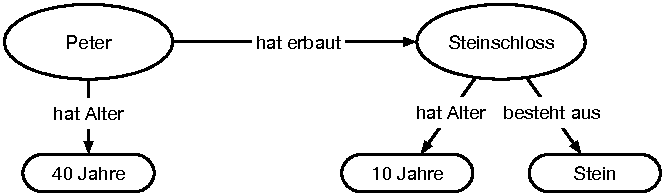
\includegraphics[width=\textwidth]{Figures/berndl/statements}
    \caption{\label{fig:statements} Informationen aus obigen Aussagen, kombiniert als Graph.}
\end{figure}

\paragraph{Linked Open Data Gedanke}

Ein weiterer Eckpfeiler des Semantic Web ist ein weiteres Konzept, das unter dem Namen \textbf{Linked Open Data - LOD} bekannt ist. Oft wird dieser Name ebenfalls für das Semantic Web selbst benutzt, die punktgenauen Definitionen überschneiden und ergänzen sich.

Einfach übersetzt zielt LOD auf öffentlich zugängliche Daten ab, die untereinander vernetzt und verlinkt sind. Somit soll es möglich sein, verteilte Datenbanken mit ihren eigenen entsprechenden Wissensbasen, miteinander zu verbinden, um so jedem Beteiligten mehr Informationen zur Verfügung zu stellen, da durch die Verlinkung einzelner Graphen ein großer Gesamtgraph entsteht. Auf diese Weise macht es Sinn, dass jede Wissensbasis ihren eigenen spezialisierten Kontext besitzt. Sollte eine Wissensbasis weitere Informationen aus einem anderen Kontext benötigen, müssen diese Daten nicht auf eigene Hand erforscht und aufbereitet werden, da eine LOD Verbindung zu einer anderen Wissensbasis hergestellt werden kann. Zur weiteren Veranschaulichung dieser Thematik und dessen Vorteile, zeigt der folgende Paragraph zwei Anwendungsfälle im geschichtswissenschaftlichen Kontext.

\paragraph{Zwei Anwendungsfälle für RDF im Geschichtswissenschaftlichen Kontext}

Ein erster Anwendungsfall, von dem geisteswissenschaftliche Wissensbasen profitieren können, ist oben bereits kurz angedeutet worden: das Verbinden einer eigenen Wissensbasis mit externen, bereits bestehenden Wissensbasen. Das Erforschen und Erkunden von Wissen benötigt generell in jeglichem Kontext sehr viel Zeit und ebenfalls Pflege der Daten. Daher kommt diesem Anwendungsfall der LOD Gedanke entgegen, da bereits erstellte Wissensbasen und deren Datenbanken öffentlich zugänglich sind.

Gerade generelle Themen oder Kontexte wie Personen, Städte oder Orte werden in vielen geschichtswissenschaftlichen Projekten benötigt, und gerade diese sind in öffentlichen Datenbanken zugänglich. Daher ist es für diese Anwendungsfälle sinnvoll, den eigens entwickelten Anwendungsfall an diese Datenbanken zu knüpfen. Dadurch wird der eigene Zeitaufwand erheblich reduziert und die angebundenen Daten genießen in der Regel außerdem einen hohen Standard, da bereits viele potenzielle Reviews von anderen Nutzern bestehen.

Ein zweiter großer Vorteil davon, geschichtswissenschaftliche Daten in Form von Metadaten und RDF zu persistieren, ist das mögliche Erschließen von vorher nicht bekannten oder erforschten Zusammenhänge der persistierten Objekte. Dazu folgendes (frei erfundenes) Beispiel: Ausgehend von der eigenen Wissensbasis, die die Daten aus \autoref{fig:statements} enthält, sollen nun zwei weitere Wissensbasen angekoppelt werden, welche auf der einen Seite weitere Informationen über Personen und vor allem deren familiärer Beziehungen beinhaltet, und auf der anderen Seite eine Wissensbasis, die mehr Informationen über Gebäude und deren Geschichte beinhaltet. Dies ist in \autoref{fig:extendedStatements} visualisiert.

\begin{figure}[htb]
    \centering
    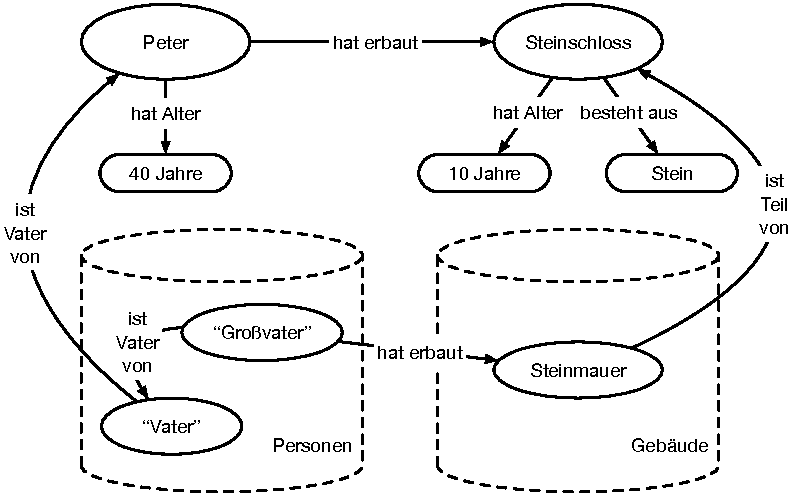
\includegraphics[width=\textwidth]{Figures/berndl/extendedStatements}
    \caption{\label{fig:extendedStatements} Grundlegende eigene Wissensbasis (oben), erweitert um zwei externe Wissensbasen (unten).}
\end{figure}

In dem Beispiel beinhaltet die eigene Wissensbasis Informationen über \q{Peter} und das \q{Steinschloss}. Durch die beiden hinzugenommenen Wissensbasen wird Peter aus dem Anwendungsbeispiel mit seinem \q{Vater}, und dieser wiederum mit seinem \q{Großvater} verbunden (die Namen sind hier zur Einfachheit ersetzt). Zudem wird die \q{Steinmauer} als ein Teil des Steinschlosses deklariert. Die beiden neuen Wissensbasen enthalten darüber hinaus bereits implizit eine eigene Verbindung, die semantisch besagt, dass der \q{Großvater} am Bau der Steinmauer beteiligt ist.

Dadurch erweitern die beiden externen Wissensbasen die eigenen Informationen durch die neu erstellten Relationen. Darüber hinaus jedoch lässt sich so ebenfalls eine neue Erkenntnis in den Daten schliessen: sowohl \q{Peter} als auch dessen \q{Großvater} sind direkt oder indirekt am Bau des \q{Steinschlosses} beteiligt.

\paragraph{Das Contextual Reference Model - CIDOC CRM}

Bisher war die technische Beschreibung der semantischen Daten im ViSIT Kontext aus Gründen der Einfachheit sehr flach gehalten. Gemäß den Semantic Web Standards basieren die Metadaten jedoch auf einem Datenmodell, um die Anforderungen des Semantic Webs zu genügen und ebenfalls technische Verabeitbarkeit zu gewährleisten.

In ViSIT ist die Wahl hierbei auf das \textbf{Contextual Reference Model CIDOC CRM} \cite{CIDOC-Doerr-2003} gefallen, da dies eine der bekanntesten und vorherrschendsten Ontologien im Bereich des kulturellen Erbes ist. Diese Ontologie wird als Basis benutzt, die im folgenden Paragraphen erweitert für den ViSIT Kontext beschrieben wird. Der größte Vorteil dieser Ontologie ist, dass sie sich nicht auf einen speziellen Bereich des kulturellem Erbes fokussiert ist, sondern auf generische Weise komplexe Zusammenhänge und verschiedene Themengebiete abbildet. Zudem solle es möglich sein, andere Ontologien oder Modelle aus dem selben Bereich in diese Ontologie zu überführen, um eine gemeinsam verständliche Wissensbasis zu kreieren.

Das CIDOC CRM wird seit mittlerweile über 10 Jahren von der CIDOC Documentation Standards Working Group\footnote{\url{http://network.icom.museum/cidoc/working-groups/overview/}} und der CIDOC CRM SIG\footnote{\url{http://network.icom.museum/cidoc/working-groups/crm-special-interest-group/}} entwickelt, welche beide Arbeitsgruppen von CIDOC\footnote{\url{http://network.icom.museum/cidoc/}} sind. Das CIDOC CRM ist 2000 als \q{Working Draft} bei der ISO/TC46/SC4\footnote{\url{https://www.iso.org/committee/48798.html}} akzeptiert worden, welcher 2006 schliesslich auch als offizieller Standard \cite{CIDOCCRM-iso21127:2006} akzeptiert wurde, und 2014 in eine überarbeitete Version \cite{CIDOCCRM-iso21127:2014} überführt wurde.

In der aktuellen Hauptversion 6.2\footnote{\url{http://www.cidoc-crm.org/Version/version-6.2}}, die im Mai 2015 veröffentlicht wurde, enthält die Ontologie 89 RDF Klassen und 149 einzigartige Relationen und Eigenschaften, die sich in einer mehrfach ineinander- sowie auseinander verzweigenden Struktur einordnen. Laufend werden ebenfalls Nebenversionen veröffentlicht - die aktuellste Versionsnummer lautet 6.2.3\footnote{\url{http://www.cidoc-crm.org/Version/version-6.2.3}}.

\paragraph{Das ViSIT Model - VisMo}

Aufbauend auf dem CIDOC CRM wurde eine Ontologie entwickelt, die den kompletten Anwendungsfall des ViSIT Projekt abbilden kann: das \textbf{ViSIT Model VisMo}. Der Fokus liegt dabei auf der Darstellung von Architektur-Objekten und Ausstellungsobjekten, die mit Personen oder Gruppen von Personen, Orten sowie zeitlichen Events in Verbindung gesetzt werden, um eine Wissensbasis zu kreieren.

Dabei erfüllt VisMo genau den Zweck, den sich das CIDOC CRM als Ziel gesetzt hat: als eine semantische \q{Erweiterung} des CIDOC CRM ist der Inhalt, der für VisMo produziert wird, direkt zum größten Teil verständlich und Leser oder Benutzer des Modells können dies intuitiver, auf der Basis der Beschreibungen des CIDOC CRM, verstehen, lesen und benutzen. Dies ist dadurch begründet, dass alle Klassen und viele der Relationen und Eigenschaften durch Vererbung speziellere Konzepte der CIDOC CRM Klassen und Relationen/Eigenschaften sind. Nur einzelne Teile des VisMo sind speziell für die Ontologie hinzugefügt worden, immer wenn kein Konzept aus dem CIDOC CRM passend für eine Vererbung war. \autoref{fig:modelworkflow} visualisiert den Entwicklungsprozess hinter VisMo.

\begin{figure}[htb]
    \centering
    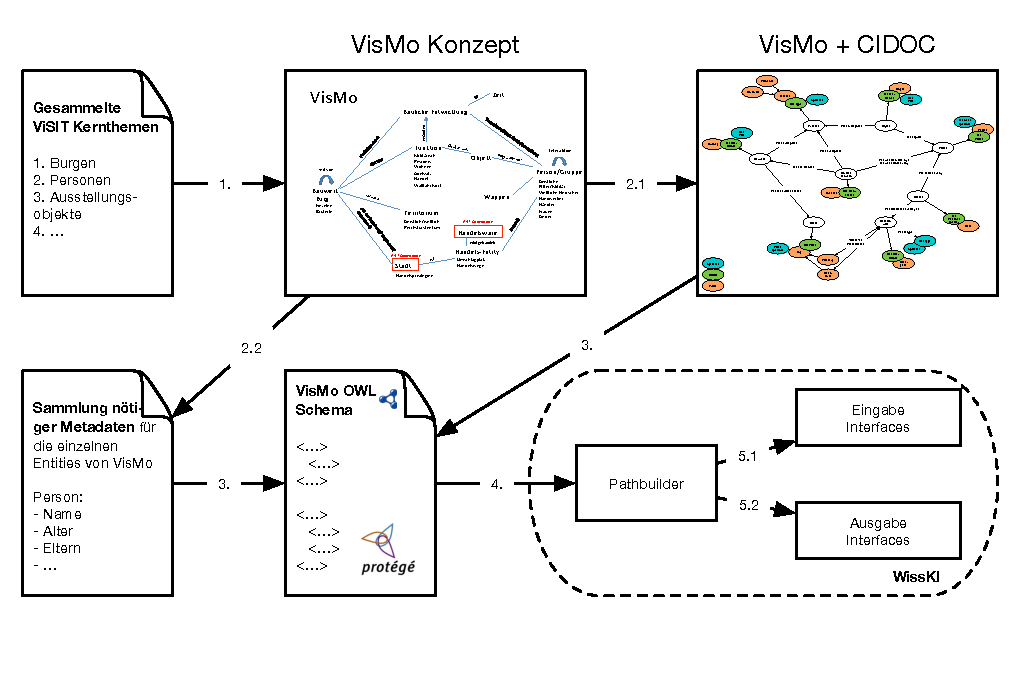
\includegraphics[width=\textwidth]{Figures/berndl/modelworkflow}
    \caption{\label{fig:modelworkflow} Arbeitsprozess hinter der Entwicklung des ViSIT Modells.}
\end{figure}

Der erste Schritt bestand dabei in der Sammlung der Kernthemen, die in ViSIT behandelt werden. Aus diesen konnte dann im nächsten Schritt ein grobes Konzept entwickelt werden, welches anschließend in RDF übertragen werden konnte. Wie oben beschrieben, wurde hierbei von CIDOC CRM Grundklassen und Relationen bzw. Eigenschaften ausgegangen, welche dann für den ViSIT Kontext erweitert und angepasst wurden. Als nächstes konnten dann die erstmals groben Konzepte und Entitäten mit benötigten Metadaten bzw. dessen Anforderungen erweitert werden. Die Ergebnisse der vorherigen Schritte konnten dann letztendlich in dem Ontologie-Editor \textbf{protegé}\footnote{\url{https://protege.stanford.edu/}} zusammengeführt werden, um eine RDF/OWL Ontologie zu erstellen. Diese ist in ihrer letzten offiziellen Version in \autoref{lst:vismo} im Appendix zu sehen.

Ebenfalls ist in \autoref{fig:modelworkflow} visualisiert, wie und an welcher Stelle die VisMo Ontologie technisch zum Einsatz kommt: sie dient als Input für das sogenannte WissKI Modul, um aus der Ontologie Ein- sowie Ausgabemasken zu generieren, welche letztendlich vom Endnutzer des ViSIT Systems benutzt werden, um einerseits Daten in die semantische Datenbank einzutragen und diese dann auch wieder auszulesen und anzuzeigen. Der große Vorteil an diesem Prozess ist, dass der Endnutzer keinerlei Wissen über das Semantic Web und seine Technologien benötigt, da der oben beschriebene Prozess davon abstrahiert. Damit schreiben und lesen die Endnutzer im Endeffekt RDF, ohne davon zu wissen. Technische Details zu diesem Prozess sowie WissKI werden in folgenden Unterkapiteln gegeben.

\subsection{Technische Details zur Semantischen Datenbank}\label{sec:technicalBackground}

infrastruktur, hosting, allgemeiner zugriff

zertifizierung, sicherheit

drupal

wisski (allgemein)

rdf4j

grundfunktionalität

\subsection{WissKI - Wissenschaftliche KommunikationsInfrastruktur}\label{sec:wisski}

aufhänger: wissenschaftlicher zugang, zugang für die geisteswissenschaftler und forscher

connection zu den rdf daten

pfade

konfiguration

\subsection{Technischer Zugang zu den Metadaten - die ViSIT REST API}\label{sec:rest}

aufhänger: technischer Zugang im gegensatz zum allgemeinen zugang

allgemeine beschreibung

\subsection{Wichtige Technische Charakteristika der Entwicklung und den Betrieb der Semantischen Datenbank}\label{sec:features}

alle sachen wie scripte und details für die lauffähige API und DB erklären 

\subsection{Zusatzfeatures - Erweiterung der Bedienbarkeit der Semantischen Datenbank}\label{sec:additional_features}

copy and paste feature

excel importer

\subsection{FAQ und häufig auftretende Probleme}\label{sec:faqSW}

drupal update

seite schaltet sich selbst in maintenance mode -> meistens ein wichtiges drupal update -> drupal per composer updaten, dann sollte wieder gehen. wenn nicht, seite per drush aus maintenance nehmen, dann ist wieder zugreifbar 







